% !TeX spellcheck = en_US 
\chapter{Introduction}
\section{Motivation}\label{intro}
As “Industrie 4.0” became the new standard, more and more data is gathered in every industry process \cite{Vogel}. By analyzing this large amount of data, new options are discovered and implemented, that can help to save resources, time, and money \cite{Theodoridis}. The use-cases range from yield improvement in chemical processes, condition monitoring in machinery, to fraud detection in banking \cite{Janiesch}. New insight from that data enables more specialized solutions and improvements in all areas of application \cite{Russell}. 

To analyze the gathered data, more and more sophisticated methods have been developed over the last few years. Not only did the available computing power take a significant leap forward, but also the methods for data-analysis and knowledge-extrapolation, that are now widely available \cite{Janiesch}. One of the most prominent methods is Machine Learning (ML) which is part of Artificial Intelligence (AI) \cite{Helm}. Since the early beginnings of AI in 1956, the idea of ML has gotten more and more attention \cite{Russell}. Today, ML is applied in all areas where traditional algorithms can not handle the amount of data or the problems are too abstract \cite{Carleo}. Image recognition or chatbots are just a small part of the possibilities ML is offering \cite{Theodoridis}.
%Especially as the computing capabilities of household computers are now far more capable and affordable. Chat-GPT is one of the latest advancements that received much public attention for the ability to interact with a human through a chat-interface and answer various questions with very precise accuracy. 

Especially Engineering sciences are interested in the implementation of ML and the associated improvement of processes \cite{Carleo}. Saving money by optimizing processes is one of the biggest driving forces for ML. In more and more use-cases, like predictive maintenance and anomaly detection, ML is the new normal \cite{Theodoridis}.

Gears are one of the most common elements in mechanical engineering and can be found in almost every part of industry applications \cite{Vullo}. Those gears are dimensioned and treated in such a way, to require the least amount of material and still fulfill their purpose without failure, throughout their desired lifetime \cite{Bugliarello}. This thesis will take a deeper look at how the application of ML can support the confidence in the calculated current state-of-damage, by specifically considering the history of the loads applied onto the gear. 
\section{Problem And Goal Formulation}
\subsection{Problem Statement}\label{prob}

In mechanical engineering, machine elements are usually designed to withstand loads in an expected range over their course of life \cite{Vietze}. Those loads are mostly not static but dynamic and can vary significantly in their magnitude over the operating time \cite{Wittel}. For example, gears in a transmission or gearbox of a car, do experience a variety of loads, depending on the torque output of the engine \cite{Yuksel}. A rapid acceleration with a heavy trailer has a different time-load profile than just cruising at constant speed.

To determine the current state-of-damage, multiple methods can be employed \cite{Lee}. One of the most used methods is the Miner rule \cite{MinerOG} (also called the Palmgren-Miner rule) which is part of the linear approaches \cite{Sun}. It is also referred to in international standards \cite{ISO1}.

One of its main advantages, is its simplicity and general applicability. The Miner rule assumes, that each load-cycle is responsible for a certain percentage of damage. Higher loads are responsible for more damage. The accumulated damage for one load is proportional to its applied cycles. A machine element is expected to fail as soon as the accumulated damage sum D reaches 1.0 (also referred to as unity) \cite{ISO1, Miller}.

When comparing this approach to experiments, it shows that the Miner rule does not always correctly calculate the true physical state-of-damage \cite{Pavlou}. For example, multiple experiments were conducted with gears, that showed that the damage sum D, calculated with Miner, is not always a reliable parameter to determine the failure point. \cite{Hanumanna}.

These different points of failure across the applied load-cycle history are not due to the natural and expected variance in the strength of the machine elements, but related to the order of applied loads \cite{Skorupa}. Depending on the order (history) of loads that are applied, gears are failing earlier than expected (before the damage sum accumulates to unity) or are capable of handling significantly more load cycles, even though the calculated accumulated damage sum exceeds 1.0  \cite{Hanumanna}.

The Miner rule completely neglects to take the variability of the order of loads into account. For that approach, it is irrelevant when a load is applied \cite{ISO1}. 
This leads to a reduced confidence in the results and thus is an unreliable prediction of the remaining service life and current state-of-damage.
The influence of the sequence of loads is very complex to capture in a simple model, since for a correct calculation, all previous cycles and loads need to be taken into account \cite{Vietze}. Even though this specific linear model has an established and proven presents in engineering, its limitations can be improved upon for a correct state-of-damage calculation.

There are other models, that are based on non-linear approaches, but are very complex and tedious to use \cite{Vietze}. Further, the general applicability is not given, as some of these approaches rely on constants that are specific to the material of the analyzed machine element \cite{Sander}.

When looking at gears specifically, the production process needs to be taken into consideration. As high-quality gears are first machined and then post-processed with heat treatment and steel ball blasting (shot peening), internal stresses are introduced that can affect the gears' ability to handle more load in a certain range than expected \cite{Benedetti}. %Or in the opposite side, make it more susceptible to specific load patterns.
Thus, not all theories are easily transferable from one machine elements to another. The current state of the art does not offer a method that can reliably predict the remaining useful life (RUL) and current state-of-damage in machine elements. The prediction of the RUL is especially difficult, as the future loads on a part are highly uncertain.


\subsection{Aim of this Thesis}
As the development of a new fatigue analysis model is out of scope for this thesis, a different approach is selected.
The aim of this thesis is to develop a method, utilizing ML, that can analyze the state-of-damage in machine elements based on the time-load history and return a confidence value of the calculated damage sum, that was acquired using a linear damage-accumulation method.
In practice, this method helps machine operators who are already having implemented methods for state-of-damage calculations, get a better understanding of how long they can expect their machines to operate. By having this method, unexpected early failures can be avoided and unnecessary maintenance stoppages reduced. 

The individual subgoals of this thesis are: the pre-processing of the available data, conceptual development of the ML-method, implementation of the method in a suitable programming language and, finally, the analysis and documentation of the results.

\section{Structure of the Thesis}
Chapter 2 gives an introduction to the topic of fatigue analysis and ML. Special attention is given to the application of ML in industrial applications. Chapter 3 presents a method that can return a confidence value for the calculated state-of-damage based on a given load-history. All the required pre-processing and necessary implementation steps are also discussed. Chapter 4 focuses on the analysis of the results. Finally, chapter 5 summarizes the results and gives an outlook on future work. 

\begin{comment}
\chapter{Überschrift} % ACHTUNG: fuer Dokumentclass FZGdasa hier \chapter verwenden (weils der Kong so will...), sonst immer \section
\label{sec:sektionsueberschrift}
%
Kapitelreferenz \chapref{sec:sektionsueberschrift} und eine Sectionsreferenz \secref{sec:paragraph} und noch ein Bild referenzieren: \figref{fig:beispiel} oder so \sfigref{fig:beispiel}
%
% ======================================================================================================
\section{Sektionsüberschrift}
\label{sec:nochmalsektion}
%
Literatur \cite{DIN3990} \cite{testweb}
%
%===================
\subsection{Subsektion}
\label{sec:subsektion}
%
\begin{figure}
	\centering
	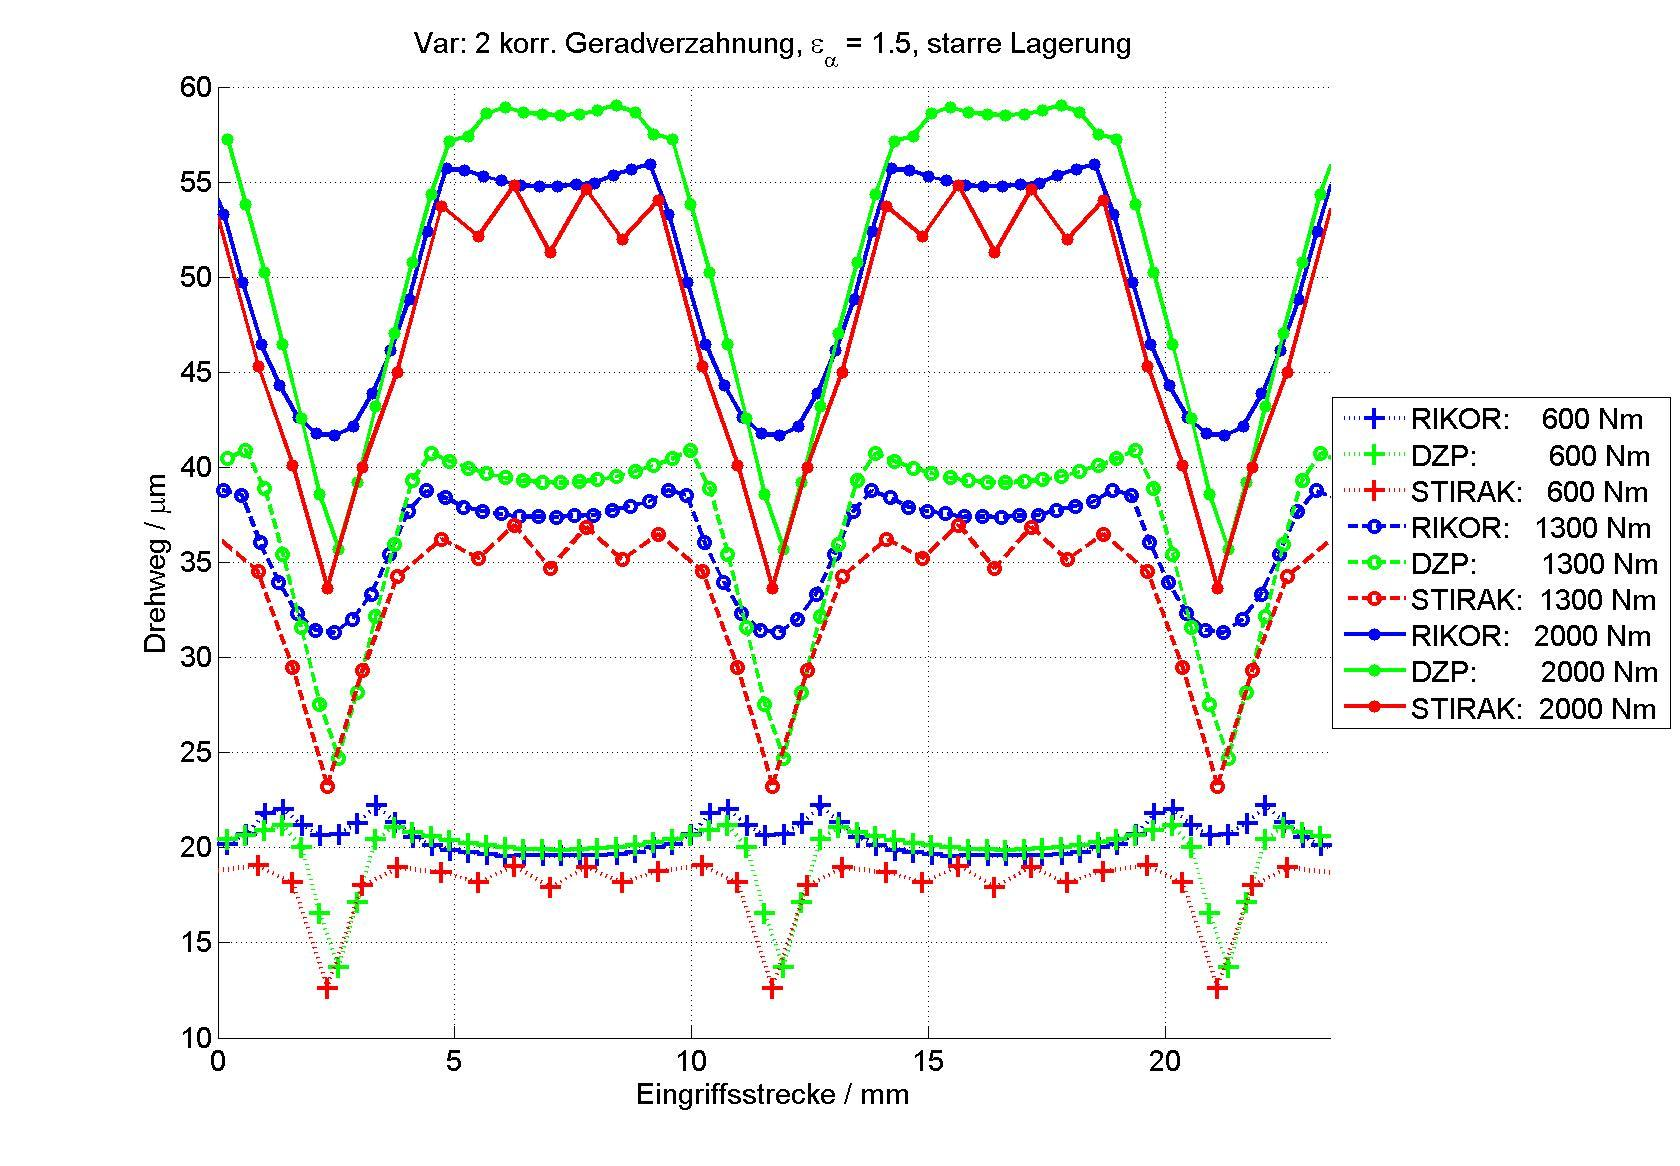
\includegraphics[width=0.5\textwidth]{_ltx/Beispiel.jpg}
	\caption{Dies ist ein wunderschönes Bild, das auch aus einer Quelle und so weiter stammen kann \cite{Niemann01}. Deshalb sind Bildunterschriften so einfach möglich.}
	\label{fig:beispiel}
\end{figure}
%
%----------------------
\subsubsection{Subsubsektion}
\label{sec:subsubsektion}
%
\textbf{fett} \textit{italic} \textsl{sl} \textsc{Kapitälchen}
%
%---------
\paragraph{Paragraph}
\label{sec:paragraph}
%
%
\newpage
\section{Formeln}
\label{sec:Formeln}
%
Das Beschreiben und Referenzieren von Formeln erfolgt nach DIN~1338.
%
\subsection{Beispiel nach DIN 1338}
%
In der Ausgleichsflächenformulierung wird der Polarwinkel über die Reihendarstellung
\begin{equation}
	\varphi_s = \sum_{j=0}^{m} \sum_{i=0}^{n} c_{ij} B_{i,n} B_{j,m}
	\label{eq:Polarwinkel}
\end{equation}
mit den Basispolynomen~$B_{i,n}$ und $B_{j,m}$ approximiert. Für die Wahl der Basispolynome eignen sich die Bernsteinpolynome
\begin{equation}
	B_{i,n}(t) = \binom{n}{i} t^i (1 - t)^{n - i}\text{,}
	\label{eq:Bernsteinpolynome}
\end{equation}
da sie die Eigenschaft der ‚Zerlegung der Eins‘ aufweisen. Die Basiskoeffizienten~$c_{ij}$ in \eqref{eq:Polarwinkel} können unter anderem mit der ‚Methode der kleinsten Fehlerquadrate‘ ermittelt werden:
\begin{equation}
	\sum_{s=1}^{q} (\varphi_s - \varphi)^2 = 0\text{.}
	\label{eq:MethodeDerKleinstenFehlerquadrate}
\end{equation}
%
\subsection{Beispiel nach DIN 1338 mit Tabelle}
%
Die Basiskoeffizienten~$c_{ij}$ in \eqref{eq:Polarwinkel} können unter anderem mit der ‚Methode der kleinsten Fehlerquadrate‘ ermittelt werden:
\begin{equation}
	\sum_{s=1}^{q} (\varphi_s - \varphi)^2 = 0\text{.}
	\label{eq:MethodeDerKleinstenFehlerquadrateMitTabelle}
\end{equation}
\begin{Gleichungsparameter}
	\Gleichungparaeintrag
		{\varphi_s}{$\mathrm{rad}$}{Polarwinkel aus\newline Punktkoordianten}
		{\varphi}{$\mathrm{rad}$}{Polarwinkel Variable}
	\Gleichungparaeintrag
		{q}{$\mathrm{-}$}{Anzahl der Punkte}
		{s}{$\mathrm{-}$}{Zählindex}
	%\Gleichungparaeintrageinfach{q}{-}{Anzahl der Punkte}
\end{Gleichungsparameter}
%
%
\newpage
\section{Dateifenster}
\label{sec:Dateifenster}
%
Referenz zu~\datref{dat:Text} mit Text.%
\begin{dateifenster}{Text}{dat:Text}
\strut
Text\\
 Text\\
Text
\strut
\end{dateifenster}
%
Referenz zu~\datref{dat:tabular} mit \texttt{tabular}.%
\begin{dateifenster}{\texttt{tabular}}{dat:tabular}
	\begin{tabular}{@{}p{2cm}@{\ }l@{\ }p{1.5cm}l@{\ }p{5cm}p{3cm}@{}}
		\multicolumn{6}{@{}l@{}}{\$ Stufe}\\
		\multicolumn{3}{@{}l}{\# Name} & \multicolumn{2}{l}{Beschreibung} & Einheit\\
		IW & = & \% \% & \# & Wellennummer & (-)\\
		IR & = & \% \% & \# & Radnnummer & (-)
	\end{tabular}
\end{dateifenster}
%
Referenz zu~\datref{dat:longtable} mit \texttt{longtable} für Seitenumbrüche.%
\begin{dateifenster}{\texttt{longtable}}{dat:longtable}
	\setlength{\LTleft}{0pt}%
	\setlength{\LTpre}{0pt}%
	\setlength{\LTpost}{0pt}%
	\begin{longtable}{@{}p{2cm}@{\ }l@{\ }p{1.5cm}l@{\ }p{5cm}p{3cm}@{}}
		\multicolumn{6}{@{}l@{}}{\$ Stufe}\\
		\multicolumn{3}{@{}l}{\# Name} & \multicolumn{2}{l}{Beschreibung} & Einheit\\
		IW & = & \% \% & \# & Wellennummer & (-)\\
		IR & = & \% \% & \# & Radnnummer & (-)\\
		... & = & \% & \# & ... & (-)\\
		... & = & \% & \# & ... & (-)\\
		... & = & \% & \# & ... & (-)\\
		... & = & \% & \# & ... & (-)\\
		... & = & \% & \# & ... & (-)\\
		... & = & \% & \# & ... & (-)\\
		... & = & \% & \# & ... & (-)\\
		... & = & \% & \# & ... & (-)\\
		... & = & \% & \# & ... & (-)\\
		... & = & \% & \# & ... & (-)\\
		... & = & \% & \# & ... & (-)\\
		... & = & \% & \# & ... & (-)\\
		... & = & \% & \# & ... & (-)\\
		... & = & \% & \# & ... & (-)\\
		... & = & \% & \# & ... & (-)\\
		... & = & \% & \# & ... & (-)\\
		... & = & \% & \# & ... & (-)\\
		... & = & \% & \# & ... & (-)\\
		... & = & \% & \# & ... & (-)\\
		... & = & \% & \# & ... & (-)\\
		... & = & \% & \# & ... & (-)\\
		... & = & \% & \# & ... & (-)\\
		... & = & \% & \# & ... & (-)\\
		... & = & \% & \# & ... & (-)\\
		... & = & \% & \# & ... & (-)\\
		... & = & \% & \# & ... & (-)\\
		... & = & \% & \# & ... & (-)\\
		... & = & \% & \# & ... & (-)\\
		... & = & \% & \# & ... & (-)
	\end{longtable}
\end{dateifenster}
\end{comment}